\documentclass[tikz,border=5pt]{standalone}
\usepackage[utf8]{inputenc}
\usepackage{amsmath}
\usepackage{tikz}
\usetikzlibrary{arrows.meta, positioning, calc, shapes.geometric}

\definecolor{seni-blue}{RGB}{0,45,98}
\definecolor{seni-red}{RGB}{206,17,38}
\definecolor{seni-gold}{RGB}{201,168,76}
\definecolor{seni-green}{RGB}{0,122,51}
\definecolor{seni-dark}{RGB}{26,26,26}

\begin{document}
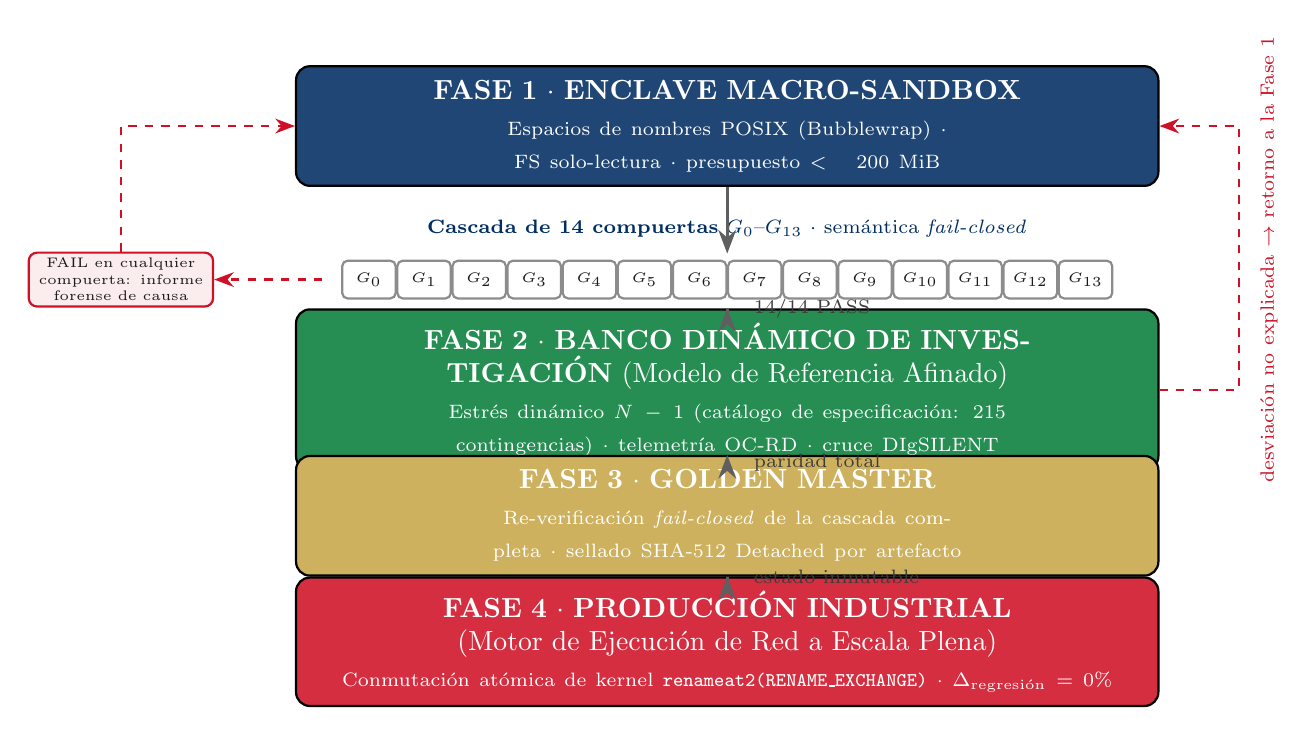
\begin{tikzpicture}[
  fase/.style={rectangle, rounded corners=5pt, draw, thick, text width=10.6cm, align=center, inner sep=5pt, minimum height=9mm},
  compuerta/.style={rectangle, rounded corners=2pt, draw=seni-dark!50, thick, fill=white, text=seni-dark, font=\tiny\bfseries, minimum width=6.8mm, minimum height=4.8mm, inner sep=0pt},
  forense/.style={rectangle, rounded corners=3pt, draw=seni-red, thick, fill=seni-red!8, text=seni-dark, font=\tiny, align=center, text width=2.2cm, inner sep=2pt},
  flujo/.style={-{Stealth[length=3mm]}, very thick, seni-dark!70},
  retorno/.style={-{Stealth[length=2.5mm]}, thick, seni-red, dashed},
  nota/.style={font=\scriptsize, text=seni-dark!85, align=center},
]
%% --- FASE 1 ---
\node[fase, fill=seni-blue!88, text=white] (f1) at (0, 0) {
  \textbf{FASE 1 $\cdot$ ENCLAVE MACRO-SANDBOX}\\[1pt]
  {\scriptsize Espacios de nombres POSIX (Bubblewrap) $\cdot$ FS solo-lectura $\cdot$ presupuesto $< 200$ MiB}
};
\node[nota, text=seni-blue] at (0, -1.30) {\textbf{Cascada de 14 compuertas} $G_0$--$G_{13}$ $\cdot$ semántica \emph{fail-closed}};
%% --- Compuertas G0..G13 (fila única) ---
\foreach \i in {0,...,13}{
  \node[compuerta] (g\i) at (-4.55+\i*0.70, -1.95) {$G_{\i}$};
}
%% --- FASE 2 ---
\node[fase, fill=seni-green!85, text=white] (f2) at (0, -3.35) {
  \textbf{FASE 2 $\cdot$ BANCO DINÁMICO DE INVESTIGACIÓN} (Modelo de Referencia Afinado)\\[1pt]
  {\scriptsize Estrés dinámico $N-1$ (catálogo de especificación: 215 contingencias) $\cdot$ telemetría OC-RD $\cdot$ cruce DIgSILENT}
};
%% --- FASE 3 ---
\node[fase, fill=seni-gold!90, text=white] (f3) at (0, -4.95) {
  \textbf{FASE 3 $\cdot$ GOLDEN MASTER}\\[1pt]
  {\scriptsize Re-verificación \emph{fail-closed} de la cascada completa $\cdot$ sellado SHA-512 Detached por artefacto}
};
%% --- FASE 4 ---
\node[fase, fill=seni-red!88, text=white] (f4) at (0, -6.55) {
  \textbf{FASE 4 $\cdot$ PRODUCCIÓN INDUSTRIAL} (Motor de Ejecución de Red a Escala Plena)\\[1pt]
  {\scriptsize Conmutación atómica de kernel \texttt{renameat2(RENAME\_EXCHANGE)} $\cdot$ $\Delta_{\text{regresión}} = 0\%$}
};
%% --- Flujo principal ---
\draw[flujo] (f1.south) -- (0, -1.62);
\draw[flujo] (0, -2.32) -- node[nota, right=2mm] {14/14 PASS} (f2.north);
\draw[flujo] (f2.south) -- node[nota, right=2mm] {paridad total} (f3.north);
\draw[flujo] (f3.south) -- node[nota, right=2mm] {estado inmutable} (f4.north);
%% --- Lazo FAIL (izquierda): informe forense y retorno a la Fase 1 ---
\node[forense] (forense) at (-7.7, -1.95) {FAIL en cualquier compuerta: informe forense de causa};
\draw[retorno] (-5.14, -1.95) -- (forense.east);
\draw[retorno] (forense.north) -- (-7.7, 0) -- (f1.west);
%% --- Lazo de desviación (derecha): retorno de la Fase 2 a la Fase 1 ---
\draw[retorno] (f2.east) -- (6.5, -3.35) -- (6.5, 0) -- (f1.east);
\node[nota, text=seni-red, rotate=90, align=center] at (6.88, -1.70) {desviación no explicada $\to$ retorno a la Fase 1};
\end{tikzpicture}
\end{document}
